Mô hình riêng biệt (Separate Ways) khi các bối cảnh bị giới hạn có quan hệ riêng biệt, không có sự phụ thuộc. Vì vậy, các bối cảnh bị giới hạn này có ngôn ngữ, mô hình, mục đích độc lập và thực thi riêng biệt. Các nhóm phát triển không phải cộng tác hay phối hợp với nhau từ đó đem lại lợi ích dễ dàng bảo trì và mở rộng hệ thống.

\begin{example} Trong miền vấn đề ngân hàng, thẻ tín dụng và khoản vay mua nhà không có mối quan hệ.

\begin{figure}[H]

\centering

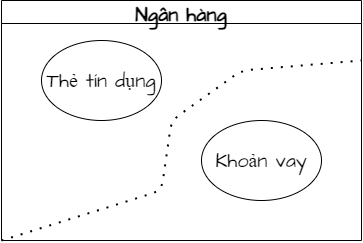
\includegraphics[scale = 0.5]{pictures/mo_hinh_rieng_biet_separate_ways/main.drawio.png}

\caption{Ví dụ mô hình riêng biệt (Separate Ways)}

\end{figure}

\end{example}

